\section{Vandermonde matrix}

The code of any shared modules for question 2 is given by:
\lstinputlisting[firstnumber=1, firstline=1, lastline=125]{2_vandermonde_matrix.py}

\subsection{a}

For this exercise, I wrote a code that firstly constructs the Vandermonde matrix $V$ for the 20 data points $x$ using that $V_{ij}=x_i^j$.
Subsequently, the LU decomposition of $V$ was found and the system $Vc=y$, for which the data points $y$ where given, was solved for $c$.
The coefficients $c$ of the corresponding 19-th degree polynomial through the data points $(x,y)$ where then used to compute and plot the values
of this polynomial for 1001 equally-spaced points within the initial range of $x$.
The corresponding result is shown in Figure \ref{fig:2a} and the computed coefficients $c$ are given as well. 

The code used is given by:
\lstinputlisting[firstnumber=127, firstline=127, lastline=167]{2_vandermonde_matrix.py}

\lstinputlisting[firstline=1, lastline=6]{vandermonde_matrix.txt}

\begin{figure}[h!]
    \centering
    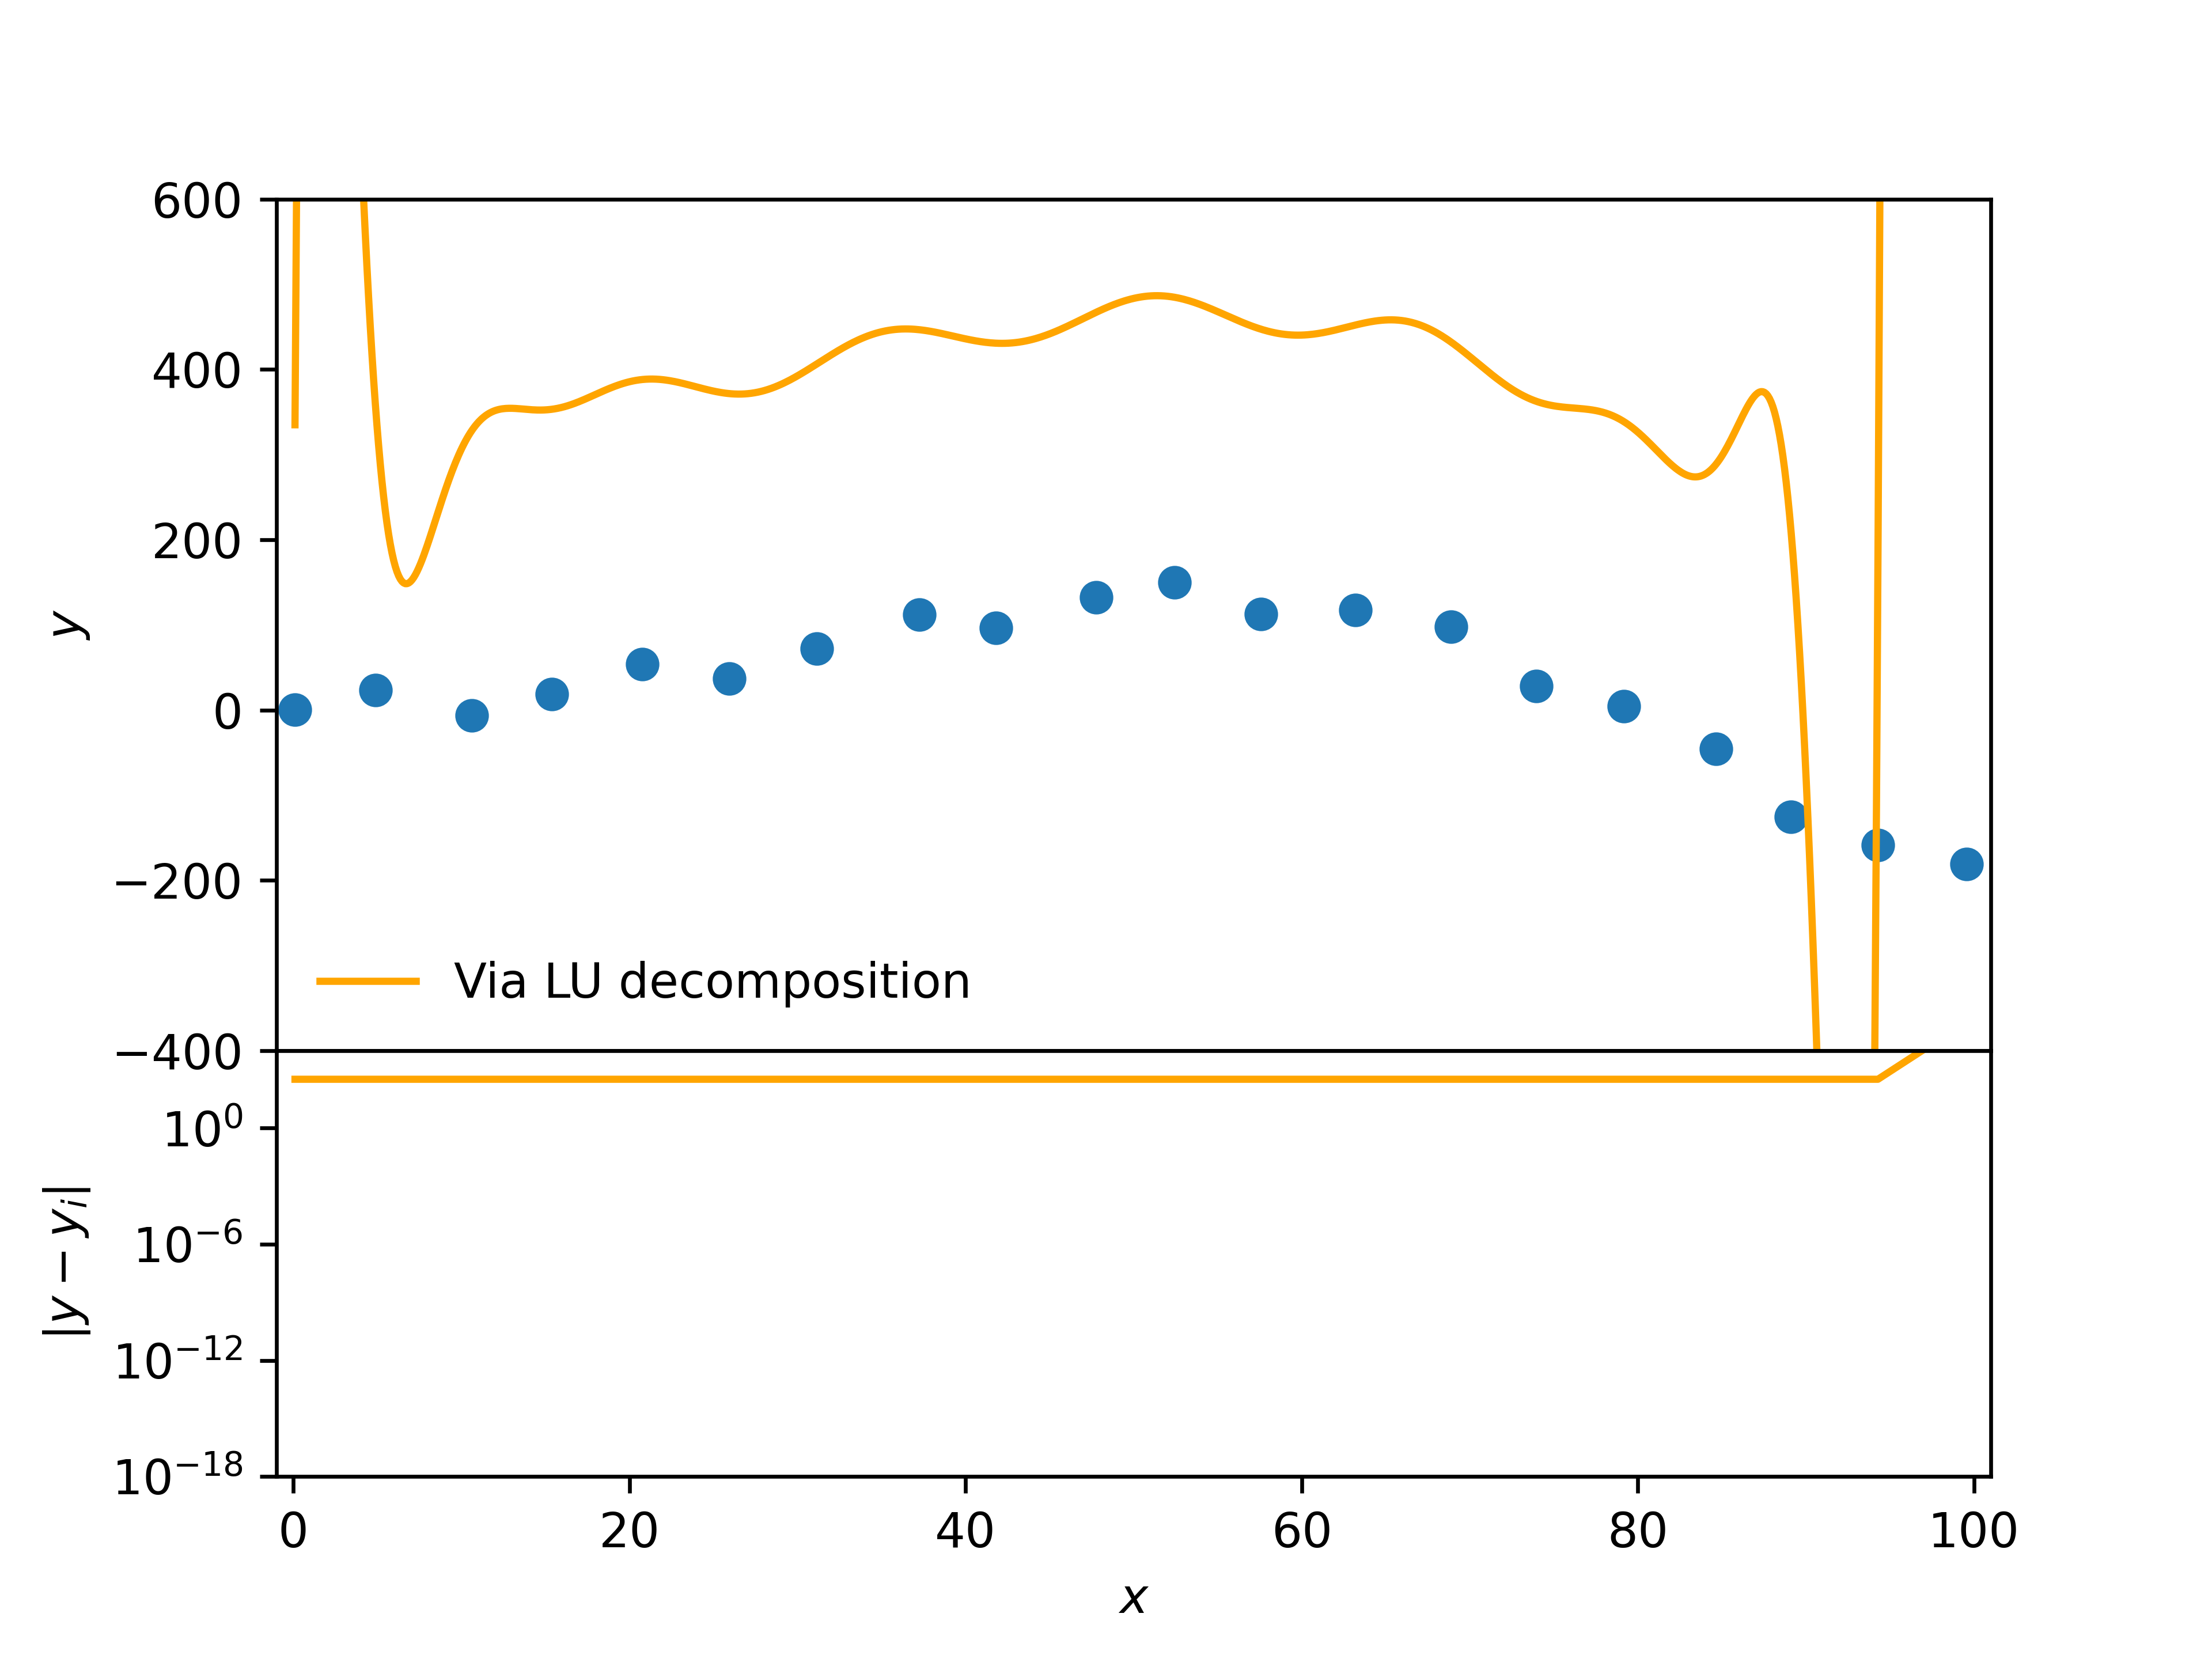
\includegraphics[width=0.9\linewidth]{./my_vandermonde_sol_2a.png}
    \caption{The original data points $(x,y)$ together with the constructed 19-th degree polynomial
    using the coefficients found by solving the system $Vc=y$ using the LU decomposition of the corresponding Vandermonde matrix are shown.
    It is clear that the polynomial does not go through the original data points, as it lies way above them. However, the shape of the polynomial does somewhat seem to follow the original data points.
    It might thus be the case that in particular the offset coefficient $c_0$ has a large error, causing the polynomial to be shifted this way. The lower panel shows the absolute difference between
    the polynomial and the data points. As we can see, this offset is about 400 which is very large.}
    \label{fig:2a}
\end{figure}

\subsection{b}

To see whether this polynomial is equal to the Lagrange polynomial, which it should be as they both go through all points and are unique, we compute the Lagrange
polynomial using Neville's algorithm on all 20 data points. Although not strictly necessary for this exercise (as M=20 and thus all points are used for the interpolation of every point),
we have implemented a bisection algorithm to find the M closest points in the data set to each interpolation value x, as this makes for a more generic Neville's algorithm which can be used
for other situations and tested for smaller M. The resulting polynomial is shown in Figure \ref{fig:2b}.

The code used is given by:
\lstinputlisting[firstnumber=169, firstline=169, lastline=185]{2_vandermonde_matrix.py}

\begin{figure}[h!]
    \centering
    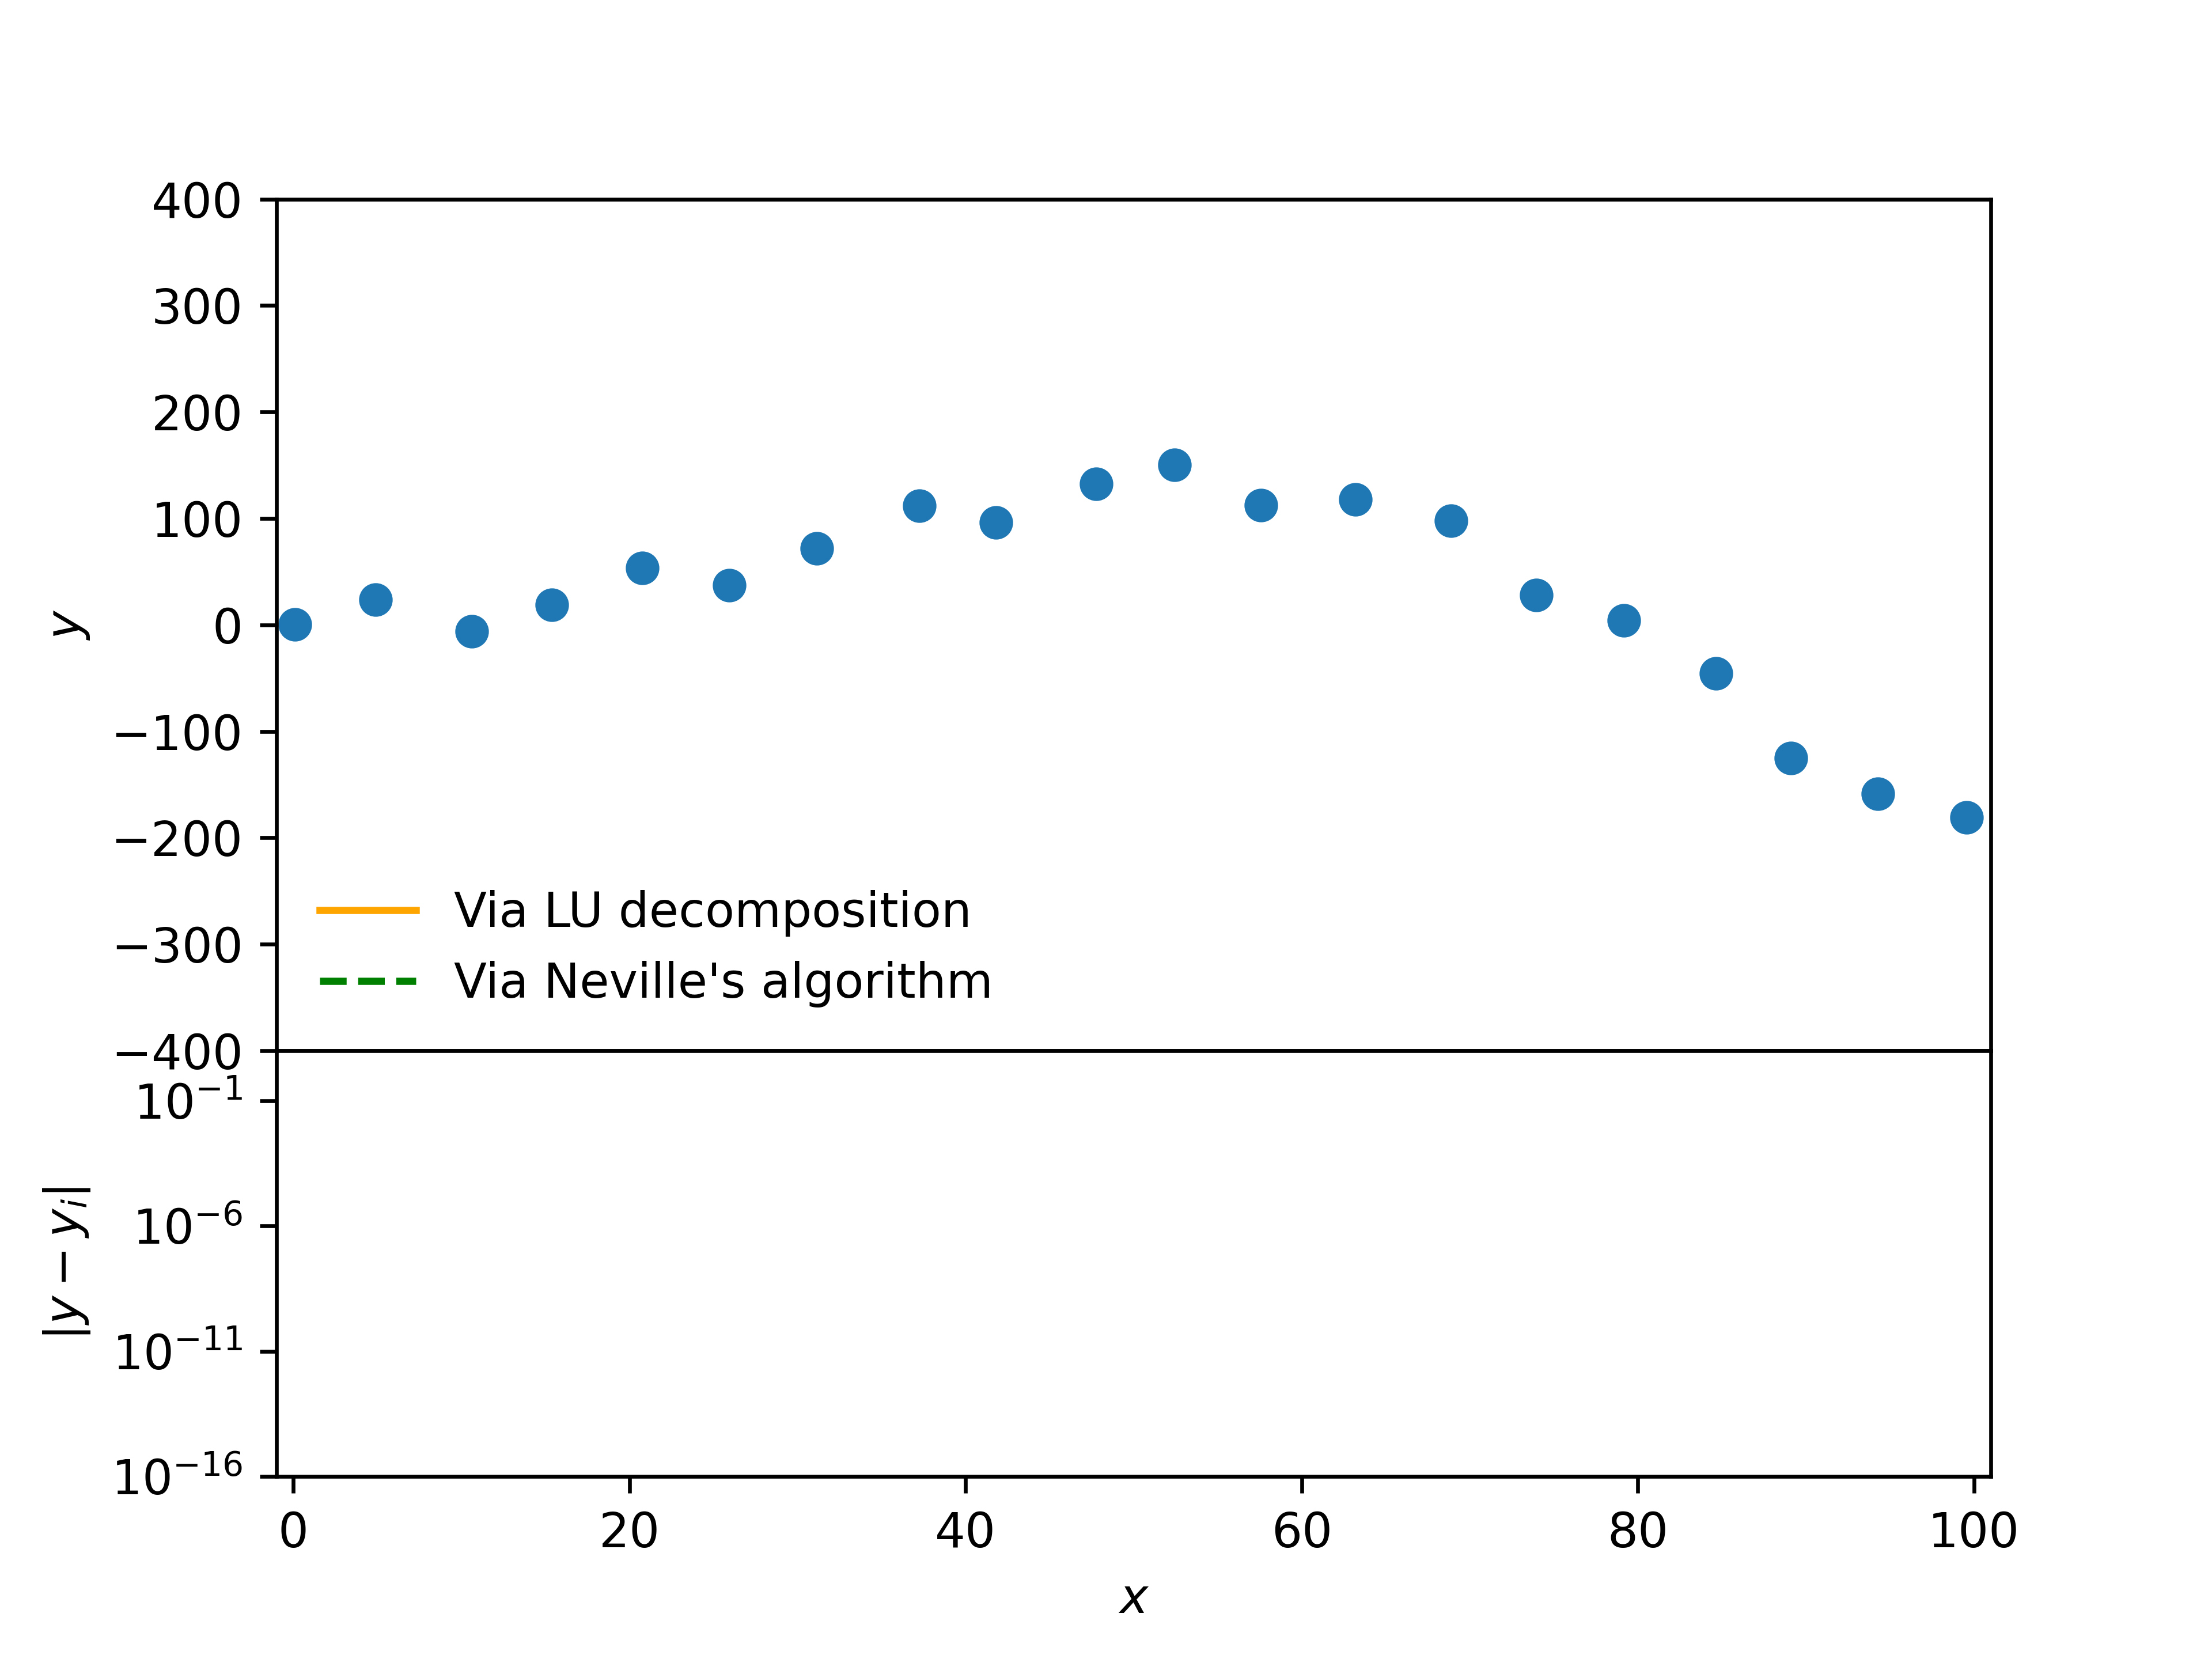
\includegraphics[width=0.9\linewidth]{./my_vandermonde_sol_2b.png}
    \caption{The previous resulting polynomial from LU decomposition is shown together with the Lagrange polynomial found using Neville's algorithm with M=20. We see that the Lagrange polynomial does closely follow the original
    data points, with a small offset shown in the lower panel of about $10^{-14}$. The offset even crashes down for some x values, indicating that the Lagrange polynomial very accurately
    follows the data points. This is to be expected, as Neville's algorithm uses direct linear interpolation on the data points, and when used on the data points themselves, the result is correct up to round off and machine error.
    The method using the Vandermonde matrix, however, is a more indirect way of computing the polynomial with more intermediate calculations, which does not compute the polynomial values directly but the polynomial coefficients first.
    As a small deviation in coefficient value can make a large difference in the polynomial values, this explains why the original LU-decomposition method gives polynomial values with a much larger error than the Lagrange polynomial from Neville's algorithm.}
    \label{fig:2b}
\end{figure}

\subsection{c}

We now try to improve the result for LU decomposition by using iterative improvements. From class we know that
$V\delta c=\delta y=Vc-y$. Thus we can now solve this system for $\delta c$ and get $c=c-\delta c$. We use both 1 and 10 iterational improvements on the coefficients and again plot the resulting polynomials.
The results are shown in Figure \ref{fig:2c}.

The code used is given by:
\lstinputlisting[firstnumber=187, firstline=187, lastline=211]{2_vandermonde_matrix.py}

\begin{figure}[h!]
    \centering
    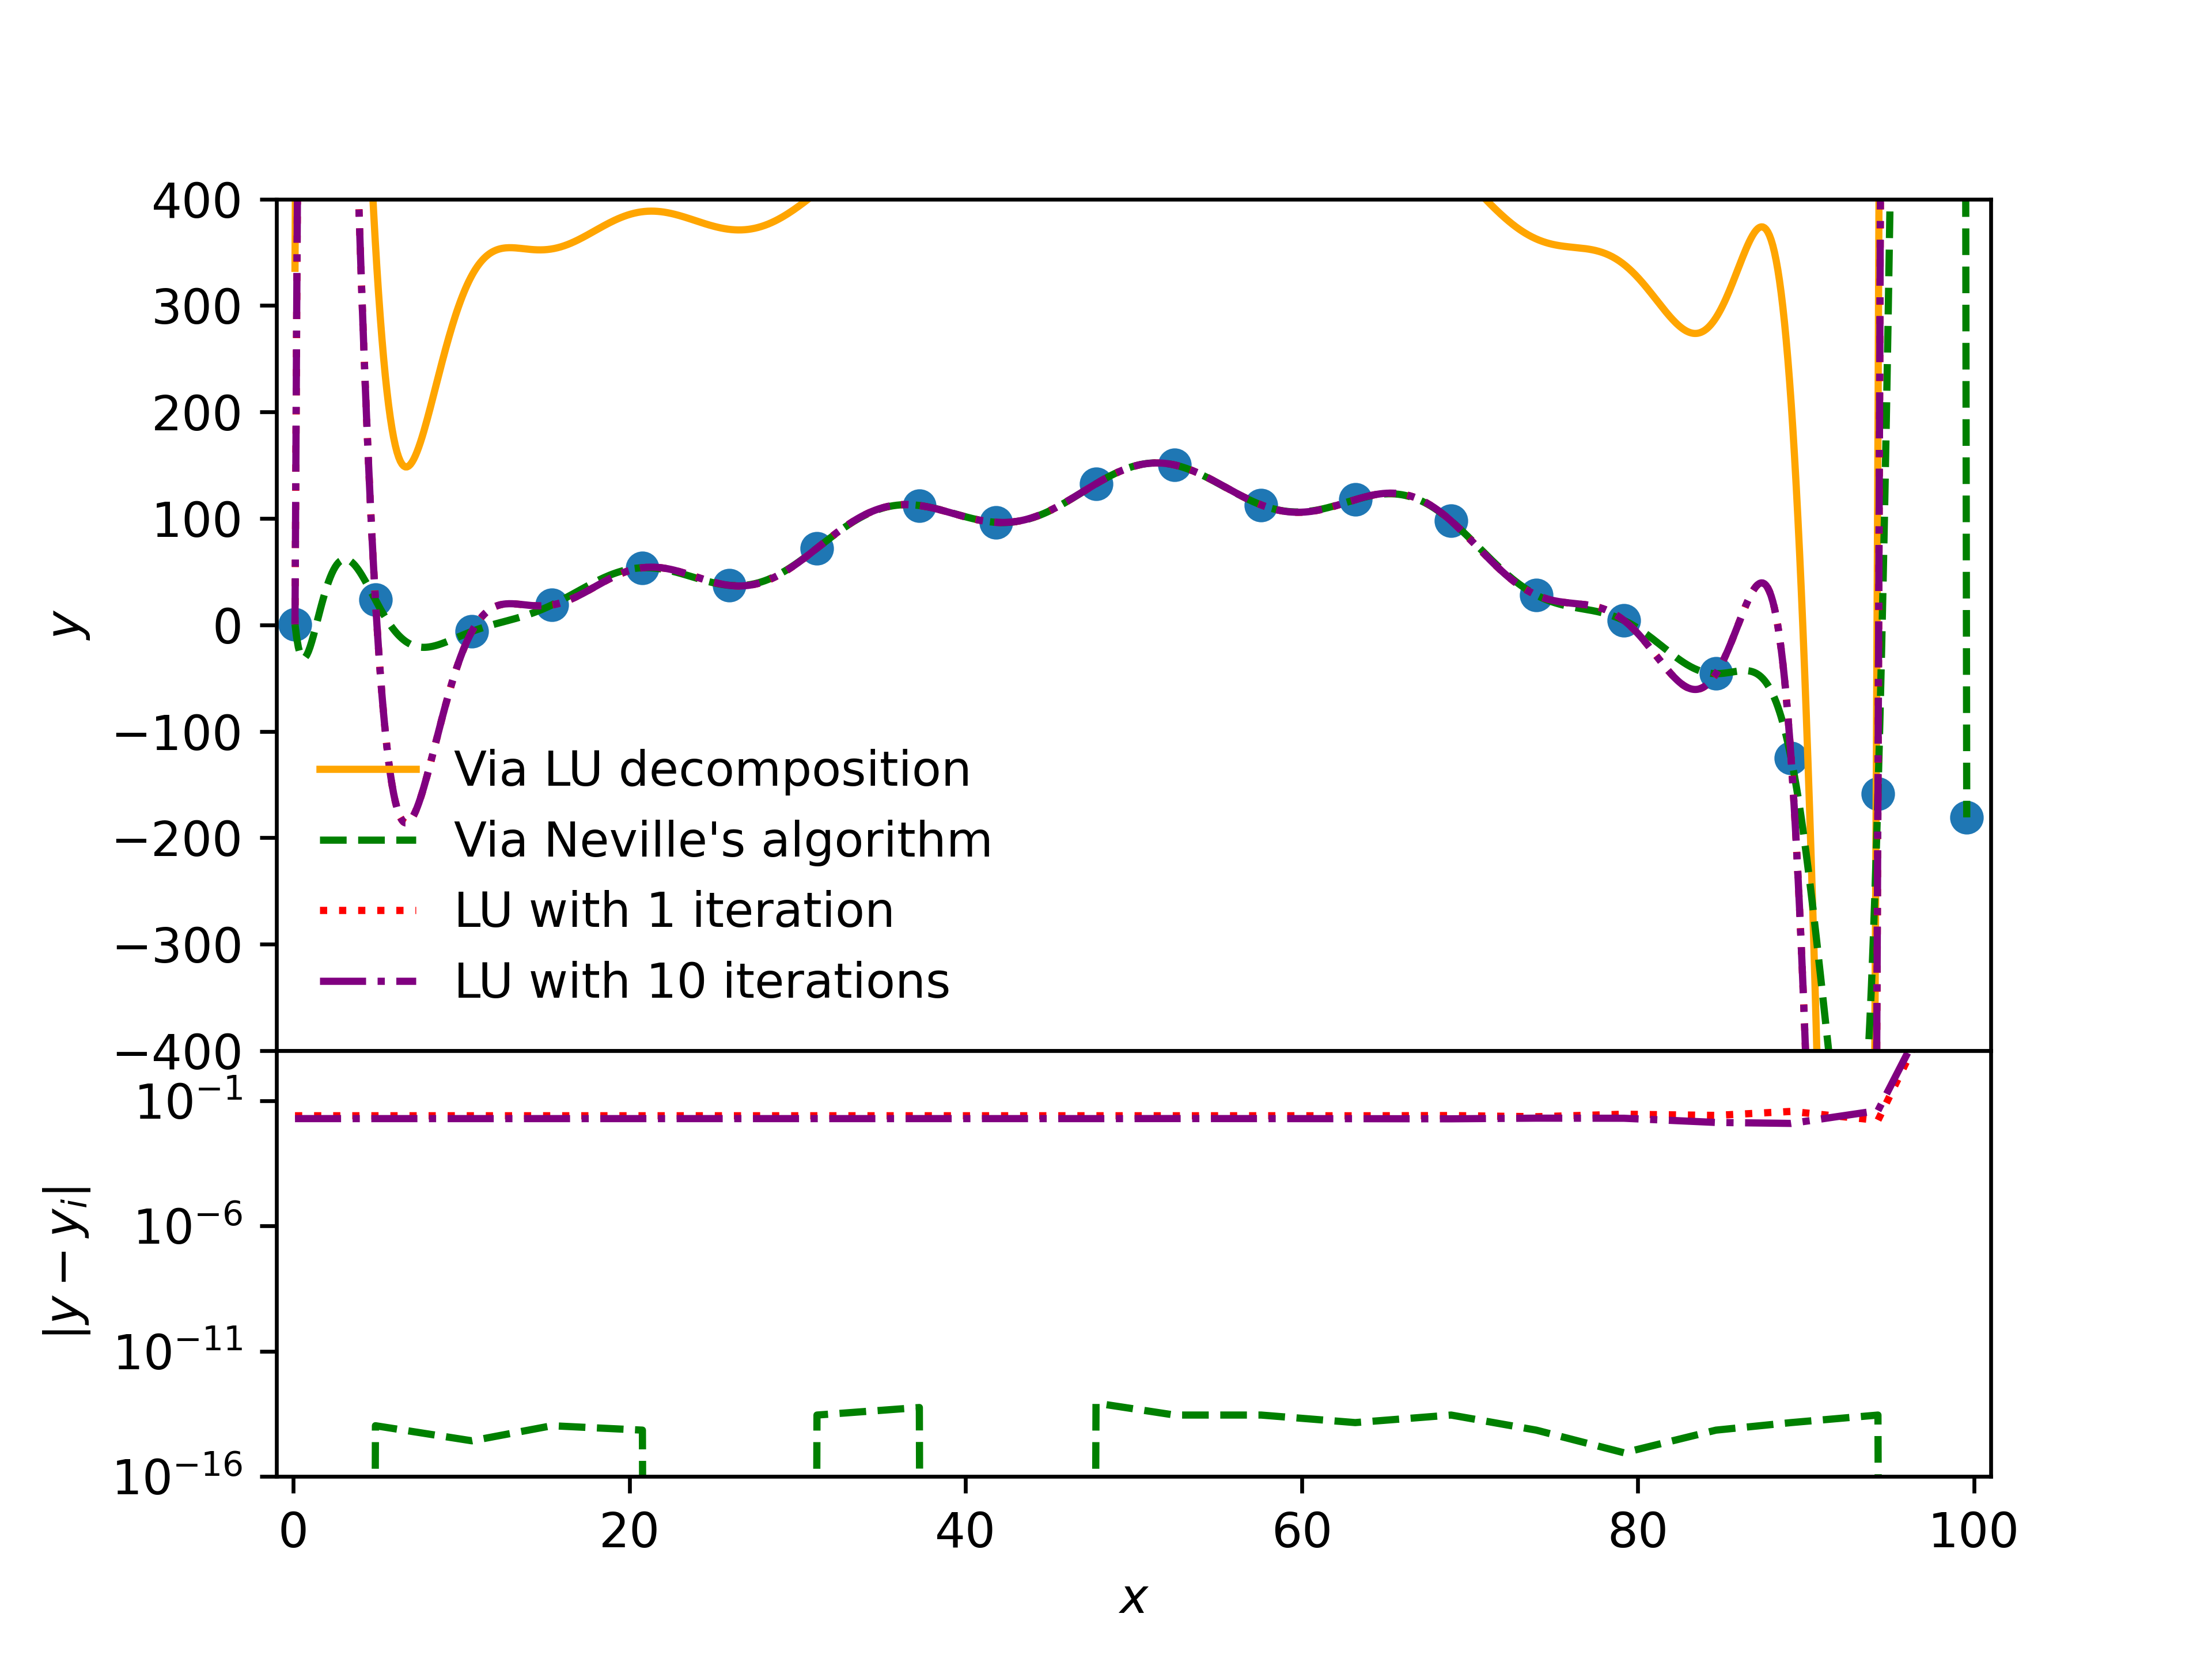
\includegraphics[width=0.9\linewidth]{./my_vandermonde_sol_2c.png}
    \caption{Again, the results from a and b are shown, but the polynomials found using 1 or 10 iterative improvements on the coefficients $c$ are added.
    We see that the first iterative improvement already greatly improves the polynomial found with LU decomposition: it now follows the data points just as the Lagrange polynomial.
    However, we do see that the offset is still larger for the improved LU polynomial compared to Neville's Lagrange polynomial. As explained previously, this can be explained by the fact that Neville's algorithm directly computes the 
    polynomial values, while the LU decomposition method computes the coefficients of the polynomial after which those are used to compute the values. This indirect way allows for more error to accumulate.
    Furthermore, we see that using 10 iterative improvements compared to only 1 does not really improve the result any more. Lastly, we note that all polynomials behave quite normally in the middle of the range of x data points,
    but more chaotic around the edges of the data points. For example, the LU decomposition polynomials do not even go through the last data point at all. It might be the case that the actual polynomial we are looking for actually behaves more chaotically around the edges,
    but this can also be a result of the way in which the polynomial is calculated. Especially in the case of Neville's algorithm, the edge points are different from the middle points, because there is no information on what is going on with the polynomial outside the edges.}
    \label{fig:2c}
\end{figure}

\subsection{d}

Lastly, we use timeit to time the execution times of a, b and c (with 10 iterations).
We have set timeit's number parameter to 1000, such that we get a more accurate run time estimate without taking more than a minute to execute.

The code used is given by:
\lstinputlisting[firstnumber=213, firstline=213, lastline=219]{2_vandermonde_matrix.py}

The resulting run times are:
\lstinputlisting[firstline=7, lastline=9]{vandermonde_matrix.txt}

We see that question b, using Neville's algorithm, uses most computation time by far. This can be explained by the fact that Neville's algorithm computes the value of the polynomial at each of 1001 different x values, directly interpolating between all the x sample points.
This requires multiple calculations for each of the 1001 interpolation points. The method using LU decomposition, however, only needs to compute the LU decomposition once and can then compute the 20 coefficients of the polynomial, which can then be used to easily compute the polynomial value for any x.
The LU decomposition method is thus more efficient. However, as we have explained before, Neville's algorithm is more accurate in the sense that it has the smallest offset caused by the fact that the method directly interpolates between the existing data points.
The LU decomposition yield a larger error because it computes the coefficients of the polynomial and not the values of the polynomial directly, causing errors to accumulate and allowing for example the found polynomial to not go through the last data point at all.